\documentclass{article}
\usepackage{ifluatex}
\ifluatex 
    \usepackage{fontspec}
    \setsansfont[
        Path = C:/Windows/Fonts/,
        Extension = .ttf ,
        BoldFont={cmunsx} ,
        ItalicFont={cmunsi} ,
        BoldItalicFont={cmunso} ,
        UprightFont={cmunss}
    ]{CMU Sans Serif}
    \setmainfont[
        Path = C:/Windows/Fonts/,
        Extension = .ttf ,
        BoldItalicFont={cmunbi} ,
        ItalicFont={cmunti} ,
        BoldFont={cmunbx} ,
        UprightFont={cmunrm}
    ]{CMU Serif}
    \setmonofont[
        Path = C:/Windows/Fonts/,
        Extension = .ttf ,
        % LightFont={cmunbtl} ,
        BoldItalicFont={cmuntx} ,
        % LightItalicFont={cmunbto} ,
        BoldFont={cmuntb} ,
        ItalicFont={cmunit} ,
        UprightFont={cmuntt}
    ]{CMU Typewriter Text}
    \defaultfontfeatures{Ligatures={TeX}}
\else
    \usepackage[T2A]{fontenc}
    \usepackage[utf8]{inputenc}
\fi
\usepackage[english,russian]{babel}
\usepackage{anyfontsize}
\usepackage{amssymb,latexsym,amsmath,amscd,mathtools,wasysym,stmaryrd}
\usepackage[shortlabels]{enumitem}
\usepackage[makeroom]{cancel}
\usepackage{graphicx}
\usepackage{geometry}
\usepackage{verbatim}
\usepackage{fvextra}

\usepackage{longtable}
\usepackage{multirow}
\usepackage{multicol}
\usepackage{tabu}
\usepackage{arydshln} % \hdashline and :
\usepackage{makecell} % \makecell for line breaks
\usepackage{tabularx}
\usepackage{xltabular}
\renewcommand\tabularxcolumn[1]{m{#1}} % for vertical centering text in X column


\usepackage{float}
\makeatletter
\g@addto@macro\@floatboxreset\centering
\makeatother
\setlength{\parindent}{0pt}
\usepackage{caption}
\usepackage{csquotes}
\usepackage[bb=dsserif]{mathalpha}
\usepackage[normalem]{ulem}

\usepackage[e]{esvect}
\let\vec\vv

\usepackage[x11names]{xcolor}
\colorlet{darkgreen}{black!25!blue!50!green}


%% Here f*cking with mathabx
\DeclareFontFamily{U}{matha}{\hyphenchar\font45}
\DeclareFontShape{U}{matha}{m}{n}{
    <5> <6> <7> <8> <9> <10> gen * matha
    <10.95> matha10 <12> <14.4> <17.28> <20.74> <24.88> matha12
}{}
\DeclareSymbolFont{matha}{U}{matha}{m}{n}
\DeclareFontFamily{U}{mathb}{\hyphenchar\font45}
\DeclareFontShape{U}{mathb}{m}{n}{
    <5> <6> <7> <8> <9> <10> gen * mathb
    <10.95> matha10 <12> <14.4> <17.28> <20.74> <24.88> mathb12
}{}
\DeclareSymbolFont{mathb}{U}{mathb}{m}{n}

\DeclareMathSymbol{\tmp}{\mathrel}{mathb}{"15}
\let\defeq\tmp
\DeclareMathSymbol{\tmp}{\mathrel}{mathb}{"16}
\let\eqdef\tmp

\usepackage{trimclip}
\DeclareMathOperator{\updownarrows}{\clipbox{0pt 0pt 4.175pt 0pt}{$\upuparrows$}\hspace{-.825px}\clipbox{0pt 0pt 4.175pt 0pt}{$\downdownarrows$}}
\DeclareMathOperator{\downuparrows}{\clipbox{0pt 0pt 4.175pt 0pt}{$\downdownarrows$}\hspace{-.825px}\clipbox{0pt 0pt 4.175pt 0pt}{$\upuparrows$}}

\makeatletter
\providecommand*\deletecounter[1]{%
    \expandafter\let\csname c@#1\endcsname\@undefined}
\makeatother


\usepackage{hyperref}
\hypersetup{
    %hidelinks,
    colorlinks=true,
    linkcolor=darkgreen,
    urlcolor=blue,
    breaklinks=true,
}

\usepackage{pgf}
\usepackage{pgfplots}
\pgfplotsset{compat=newest}
\usepackage{tikz,tikz-3dplot}
\usepackage{tkz-euclide}
\usetikzlibrary{calc,automata,patterns,angles,quotes,backgrounds,shapes.geometric,trees,positioning,decorations.pathreplacing}
\usetikzlibrary{lindenmayersystems}
\pgfkeys{/pgf/plot/gnuplot call={cd Output && gnuplot}}
\usepgfplotslibrary{fillbetween,polar}
\usetikzlibrary{quotes,babel}
\ifluatex
\usetikzlibrary{graphs,graphs.standard,graphdrawing}
\usegdlibrary{layered,trees,circular,force}
\else
% \errmessage{Run with LuaTeX, if you want to use gdlibraries}
\fi
\makeatletter
\newcommand\currentnode{\the\tikz@lastxsaved,\the\tikz@lastysaved}
\makeatother

%\usepgfplotslibrary{external} 
%\tikzexternalize

\makeatletter
\newcommand*\circled[2][1.0]{\tikz[baseline=(char.base)]{
        \node[shape=circle, draw, inner sep=2pt,
        minimum height={\f@size*#1},] (char) {#2};}}
\makeatother

\newcommand{\existence}{{\circled{$\exists$}}}
\newcommand{\uniqueness}{{\circled{$\hspace{0.5px}!$}}}
\newcommand{\rightimp}{{\circled{$\Rightarrow$}}}
\newcommand{\leftimp}{{\circled{$\Leftarrow$}}}

\DeclareMathOperator{\sign}{sign}
\DeclareMathOperator{\Cl}{Cl}
\DeclareMathOperator{\proj}{pr}
\DeclareMathOperator{\Arg}{Arg}
\DeclareMathOperator{\supp}{supp}
\DeclareMathOperator{\diag}{diag}
\DeclareMathOperator{\tr}{tr}
\DeclareMathOperator{\rank}{rank}
\DeclareMathOperator{\Lat}{Lat}
\DeclareMathOperator{\Lin}{Lin}
\DeclareMathOperator{\Ln}{Ln}
\DeclareMathOperator{\Orbit}{Orbit}
\DeclareMathOperator{\St}{St}
\DeclareMathOperator{\Seq}{Seq}
\DeclareMathOperator{\PSet}{PSet}
\DeclareMathOperator{\MSet}{MSet}
\DeclareMathOperator{\Cyc}{Cyc}
\DeclareMathOperator{\Hom}{Hom}
\DeclareMathOperator{\End}{End}
\DeclareMathOperator{\Aut}{Aut}
\DeclareMathOperator{\Ker}{Ker}
\DeclareMathOperator{\Def}{def}
\DeclareMathOperator{\Alt}{Alt}
\DeclareMathOperator{\Sim}{Sim}
\DeclareMathOperator{\Int}{Int}
\DeclareMathOperator{\grad}{grad}
\DeclareMathOperator{\sech}{sech}
\DeclareMathOperator{\csch}{csch}
\DeclareMathOperator{\asin}{\sin^{-1}}
\DeclareMathOperator{\acos}{\cos^{-1}}
\DeclareMathOperator{\atan}{\tan^{-1}}
\DeclareMathOperator{\acot}{\cot^{-1}}
\DeclareMathOperator{\asec}{\sec^{-1}}
\DeclareMathOperator{\acsc}{\csc^{-1}}
\DeclareMathOperator{\asinh}{\sinh^{-1}}
\DeclareMathOperator{\acosh}{\cosh^{-1}}
\DeclareMathOperator{\atanh}{\tanh^{-1}}
\DeclareMathOperator{\acoth}{\coth^{-1}}
\DeclareMathOperator{\asech}{\sech^{-1}}
\DeclareMathOperator{\acsch}{\csch^{-1}}

\newcommand*{\scriptA}{{\mathcal{A}}}
\newcommand*{\scriptB}{{\mathcal{B}}}
\newcommand*{\scriptC}{{\mathcal{C}}}
\newcommand*{\scriptD}{{\mathcal{D}}}
\newcommand*{\scriptF}{{\mathcal{F}}}
\newcommand*{\scriptG}{{\mathcal{G}}}
\newcommand*{\scriptH}{{\mathcal{H}}}
\newcommand*{\scriptK}{{\mathcal{K}}}
\newcommand*{\scriptL}{{\mathcal{L}}}
\newcommand*{\scriptM}{{\mathcal{M}}}
\newcommand*{\scriptP}{{\mathcal{P}}}
\newcommand*{\scriptQ}{{\mathcal{Q}}}
\newcommand*{\scriptR}{{\mathcal{R}}}
\newcommand*{\scriptT}{{\mathcal{T}}}
\newcommand*{\scriptU}{{\mathcal{U}}}
\newcommand*{\scriptX}{{\mathcal{X}}}
\newcommand*{\Cnk}[2]{\left(\begin{matrix}#1\\#2\end{matrix}\right)}
\newcommand*{\im}{{\mathbf i}}
\newcommand*{\id}{{\mathrm{id}}}
\newcommand*{\compl}{^\complement}
\newcommand*{\dotprod}[2]{{\left\langle{#1},{#2}\right\rangle}}
\newcommand\matr[1]{\left(\begin{matrix}#1\end{matrix}\right)}
\newcommand\matrd[1]{\left|\begin{matrix}#1\end{matrix}\right|}
\newcommand\arr[2]{\left(\begin{array}{#1}#2\end{array}\right)}

\DeclareMathOperator{\divby}{\scalebox{1}[.65]{\vdots}}
\DeclareMathOperator{\toto}{\rightrightarrows}
\DeclareMathOperator{\ntoto}{\not\rightrightarrows}

\newcommand{\bigmid}{\mathrel{\big|}}
\newcommand{\Bigmid}{\mathrel{\Big|}}
\newcommand{\biggmid}{\mathrel{\bigg|}}

\newcommand{\undercolorblack}[2]{{\color{#1}\underline{\color{black}#2}}}
\newcommand{\undercolor}[2]{{\colorlet{tmp}{.}\color{#1}\underline{\color{tmp}#2}}}

\usepackage{adjustbox}

\geometry{margin=1in}
\usepackage{fancyhdr}
\pagestyle{fancy}
\fancyfoot[L]{}
\fancyfoot[C]{Иванов Тимофей}
\fancyfoot[R]{\pagename\ \thepage}
\fancyhead[L]{}
\fancyhead[R]{\leftmark}
\renewcommand{\sectionmark}[1]{\markboth{#1}{}}

\setcounter{tocdepth}{5}
\usepackage{amsthm}
\usepackage{chngcntr}

\theoremstyle{definition}
\newtheorem{definition}{Определение}
\counterwithin*{definition}{section}

\theoremstyle{plain}
\newtheorem{theorem}{Теорема}
\counterwithin*{theorem}{section} % Without changing appearance
\newtheorem{lemma}{Лемма}
\counterwithin*{lemma}{section}
\newtheorem{corollary}{Следствие}[theorem]
\counterwithin{corollary}{theorem} % Changing appearance
\counterwithin{corollary}{lemma}
\newtheorem*{claim}{Утверждение}
\newtheorem{property}{Свойство}[definition]

\theoremstyle{remark}
\newtheorem*{remark}{Замечание}
\newtheorem*{example}{Пример}

\newtheorem*{discourse}{Рассуждение}


%\renewcommand\qedsymbol{$\blacksquare$}

\counterwithin{equation}{section}

\input{Headers/graphs}

\usepackage[outputdir=Output, cache=false]{minted}

\begin{document}
    \begin{itemize}
        \item Exploratory DA~--- анализ (чаще всего глазками) данных, чтобы найти в нём пропуски, выбросы и прочий мусор, который вы можете глазами найти. Тут же вы думаете о том, чем эти данные являются, и как их хранить. А ещё тут вы можете формировать базовые гипотезы.
        \item Confirmatory DA~--- не рассказали, что такое.
        \item Показательный анализ данных~--- машинное обучение с целью что-нибудь предсказывать.
        \item Визуализация данных.
    \end{itemize}
    Знание~--- закономерность в некоторой области, которые позволяют решать проблемы.\\
    Data Mining~--- один из этапов в извлечении знаний из данных. Тут три этапа:
    \begin{enumerate}
        \item Сбор данных.
        \item Выделение признаков.
        \item Применение ML.
    \end{enumerate}
    Фактически это как DA, но с акцентом на немного другое.\\
    Data Science:
    \begin{itemize}
        \item Сбор данных.
        \item Интеграция данных (data integration).
        \item Хранение данных (data warehousing).
        \item Анализ данных.
        \item Высокопроизводительные вычисления (high-performance computing).
    \end{itemize}
    Как это с точки зрения бизнеса выглядит? Есть CRISP-DM:
    \begin{enumerate}
        \item Понимание бизнеса (перевод слов заказчика на что-то понятное).
        \item Понимание данных (требование правильных данных от заказчика).
        \item Подготовка данных (понять, как хранить данные).
        \item Моделирование (собственно, решать задачу).
        \item Оценка (понять, что мы получили).
        \item Если всё хорошо, внедряем, заворачиваем в красивую обёртку и т.п.
    \end{enumerate}
    \paragraph{Данные.}
    Данные бывают структурированные, неструктурированные и частично структурированные. Чаще всего мы встречаем неструктурированные. Это видео, посты в соцсетях и любая другая хрень, которую мы встречаем. Частично структурированные~--- XML, JSON и прочий мусор, который до полностью структурированных не дотягивает. А полностью структурированные данные~--- это матрицы (из $n$ объектов по $m$ характеристик у каждого).\\
    Имея неструктурированные или частично структурированные данные, мы почти всегда хотим его структурировать, чтобы было удобнее.\\
    В DA строку матрицы называют object, instance, sample, example и как угодно ещё, а столбец матрицы~--- feature, attribute, characteristic или factor.\\
    Что важно про наши матрицы? Чтобы порядок столбцов и строк был не важен. Если ваш алгоритм не такой, это странно. Исключение: временной ряд.
    \paragraph{Признаки.}
    Глобально их два: категория и число (качество и количество). Первое дискретно, второе непрерывно, категории мы можем только на равенство проверять, а с числами можем арифметику делать. Категориям обычно целое число сопоставляют, чтобы удобно было. Но есть и другие типы, например, порядковый: дискретный, но есть порядок. Впрочем, очень часто он сводится к либо к категории, либо к числу.\\
    С числами работать гораздо удобнее, но если надо, легко можно дискретизировать наше число любом образом (например, баллы в оценку~--- дискретизация). Как преобразовать порядковый тип во что-то? Можно преобразовать в число через порядковый номер. А можно в категорию, создав $k$ бинарных значений вида ${}<x$.\\
    \subparagraph{One-hot encoding.}
    Берём категорию из $k$ значений, преобразуем в $k$ булевых категорий вида ${}=c_i$, а потом из истины сделать 1, а из лжи~--- 0. Отличный план, как из категории сделать число.\\
    Ещё можно преобразовывать иначе, например категории сопоставлять случайный вектор или число, бинарное представление которого используется как новые признаки.\\
    Важное примечание: числа~--- не всегда числа. Например, если мы цифры распознаём, то плохо считать числа числами, а не категориями. Потому что изображение тройки не находится между изображением двойки и четвёрки. Поэтому аккуратно с преобразованием категорий в числа.\\
    Ещё интересность: время. Если у нас есть периоды, то хреначим синус и косинус, чтобы периодично было:
    \[
    f_{2e-1}=\sin\frac{2\pi t}{T_e}\qquad\qquad f_{2e}=\cos\frac{2\pi t}{T_e}
    \]
    Или ещё интересность, цвет. Цвет кодируем в RGB, а не в HSV/HSB, потому что там тон цвета неоднозначный. Красный~--- это и 0, и 360.\\
    Как хранить данные? Самый простой формат: CSV. Он плохо стандартизирован, правда. А ещё его недостаток в том, что там шапки нет. Нет ни информации о типах, ничего. Если хочется более человеческого~--- ARFF: примерно как CSV, но более стандартизирован и имеет шапку с типами данных. Типы: Numeric (число), Nominal (категория), String и Date.
    \begin{figure}[H]
        \centering
        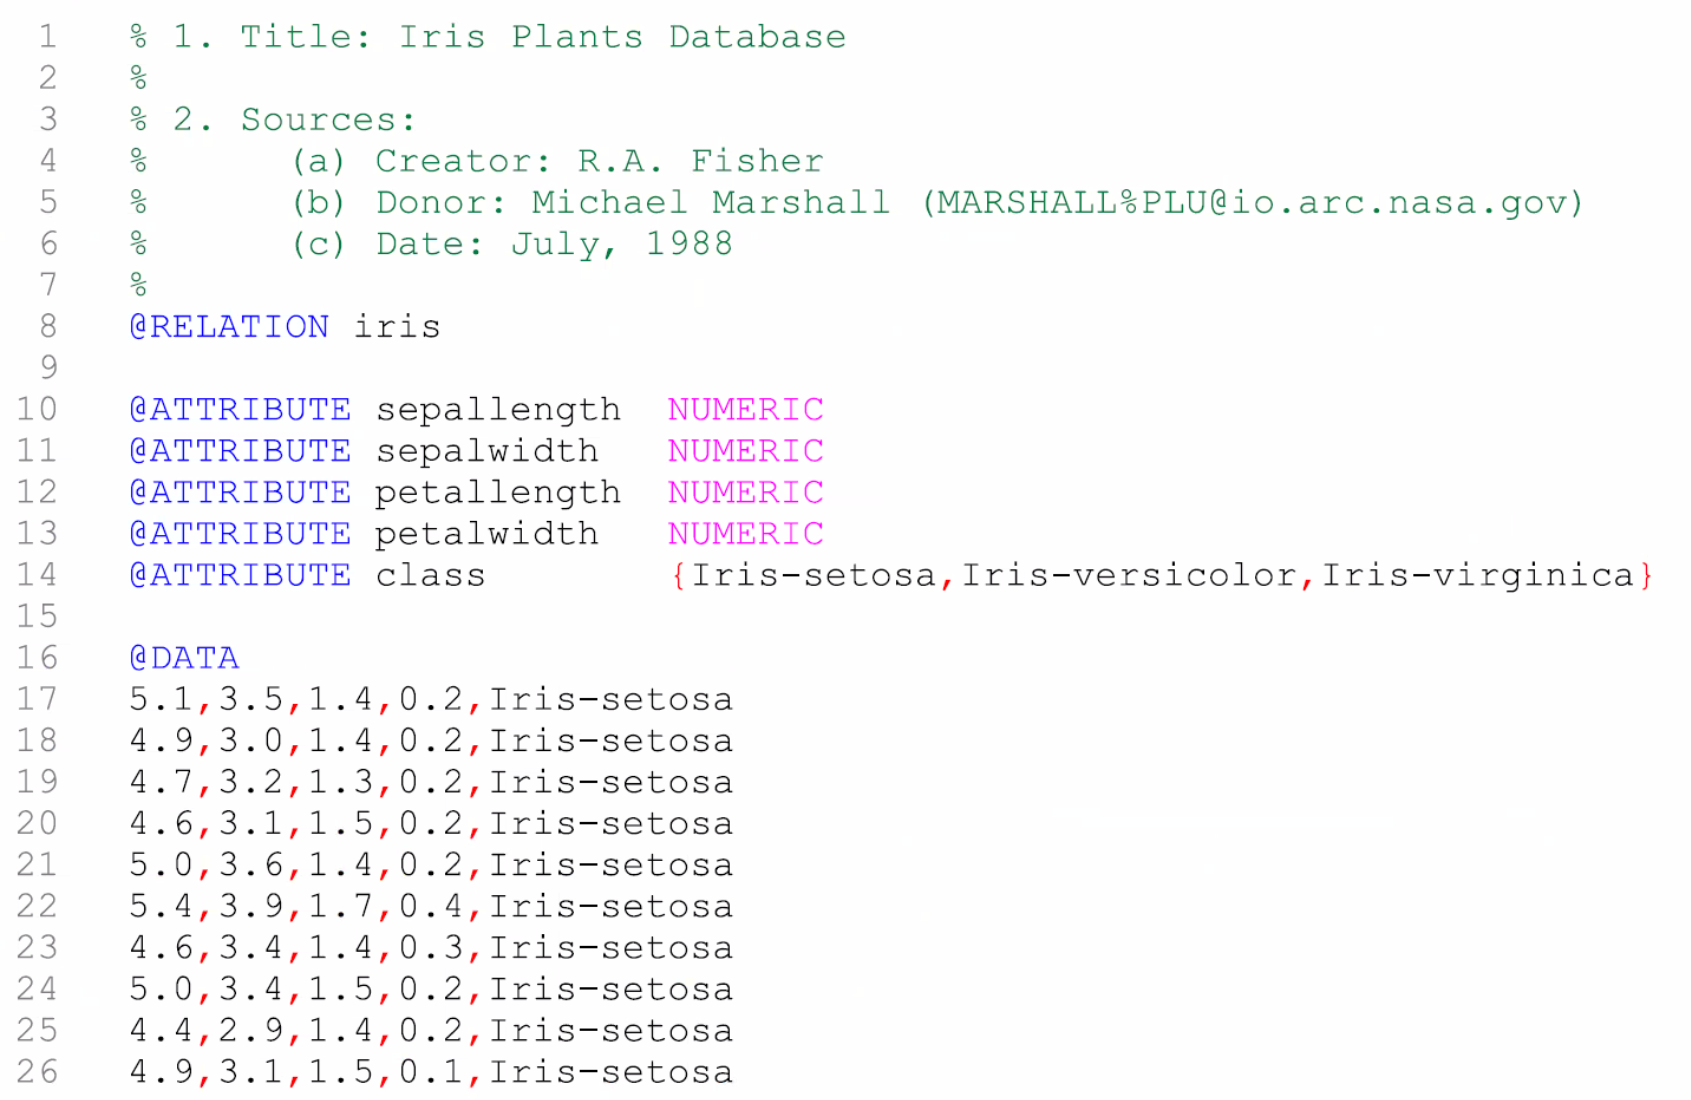
\includegraphics[width=0.9\linewidth]{Images/ARFF-example}
        \label{fig:arff-example}
    \end{figure}\noindent
    Прочие типы данных.
    \begin{itemize}
        \item Картинка. Самое простое~--- двух- (или трёх-)мерная матрица. И есть 1000 алгоритмов, как привести её в один вектор (притом довольно маленький).
        \item Текст. Тут сложнее. Самое тупое~--- посчитать частоту слов. Но не надо, тут сразу двигайте в сторону LLM.
        \item Звук. Это сигнал во времени, и самый простой вариант его представить~--- вектор значений. Для него тоже есть всякие штуки типа спектрограммы Мэла, чтобы преобразовывать звук во что-то более адекватное.
        \item Видео. Это мультимодальный объект, то есть объект, в котором разные типы внутри. Их анализировать тоже своими методами.
    \end{itemize}
    \paragraph{Нормализация.} Зачем? Чтобы признаки с большей дисперсией не влияли на результат сильнее остальных.\\
    Как? Сначала отбросим единицы измерения. Чтобы это было корректно, алгоритм должен быть инвариантен относительно линейных преобразований над признаками. А дальше надо как-то нормализовать дисперсию. Можно, например, вычесть из каждого признака минимум и поделить на разность между максимумом и минимумом. Это $[0;1]$-масштабирование. А ещё можно вычесть (выборное) мат. ожидание из признака и поделить на (выборное) стандартное отклонение это Z-масштабирование. Способов ещё куча, но это два простых.\\
    Как жить с ситуацией, когда у нас признаки зависимы? Никак не жить, если так, вы плохо собрали данные.
    \paragraph{Веса и сэмплирование.}
    Отлично, мы всё нормализовали, а теперь у нас из специфики задачи какие-то признаки более важны. Или могут быть объекты более важны.\\
    Говорят, что объект/признак обладает весом $w$, если он в $w$ раз больше влияет на результат. Если $w$ целое, то это эквивалентно тому, что объект/признак встречается $w$ раз.\\
    Примеры: учёт веса признака
    \[
    \operatorname{dist}(a;b)=\sqrt{\sum\limits_{j=1}^mw_j(a_j-b_j)^2}
    \]
    учёт веса объекта:
    \[
    \mathfrak L_D(\theta)=\sum\limits_{x\in D}w(x)\mathfrak L(x;\theta)
    \]
    А есть сэмплирование: вместо вхождения кучу раз в датасет мы можем сэмплировать объекты с вероятностью $\frac{w_j}{\sum w_j}$.\\
    Ещё это может использоваться для балансировки. Если вы знаете, что реальное распределение не очень сочетается с распределением данных, то мы можем пореже выбирать объекты мажоритарного класса или почаще объекты миноритарного класса (например, в данных одна группа большая, а другая~--- маленькая, а в жизни они равны, и мы даём большие веса малой группе). Да и в принципе, если нас не интересует распределение признаков по классам, распределение будет чаще подсовывать вам штуки из мажоритарного класса, что вам не всегда хочется.\\
    Как сэмплировать? Можно рандомно, можно каждый $x$-тый объект (систематически), можно стратифицированно (ровно в соотношение с какой-то категорией), можно кластерное (если кто-то уже за нас разбил объекты на множества, их множеств можно выбрать несколько).
    \paragraph{Шум.}
    Аномалии~--- плохие объекты для модели. Ошибки~--- плохие объекты для реальности. Пример: пусть у нас есть расход топлива автомобилями. И у нас у одного указан 30л / 100км. Если это грузовой автомобиль, а остальные~--- легковые, то это аномалия. А если объект всем хорош, и данные такие, то это ошибка (а возникнуть такое могло из-за того, что кто-то подразумевал мили на галлон).\\
    Пропуски в наборе данных. Откуда? Из склейки разных наборов данных, из изначально херовых данных или откуда угодно ещё. В CSV нет стандартного способа это обозначить, в ARFF это вопросик, а ещё можно специальное значения: None/Null для строк, категория с несуществующим номером для категорий или NaN для числа. Что делать с этим? Вырезать (признак или объект), заменить (заполнить пропуск средним арифметическим/модой/алгоритмом предсказания, который умеет в пропуски) или добавить (добавить новый признак, который говорит, были ли пропуск или нет; если там была категория, можно отдельное значение категории туда добавить, а не новое свойство делать).
    \\\\\\
    \section{Терминология.}
    \paragraph{Виды искусственного интеллекта.}
    \begin{itemize}
        \item \textbf{Слабый (узкий) ИИ}. Нацелен на решение специфичной задачи, причем способ ее решения не подходит для решения других задач.
        \item \textbf{Сильный (общий) ИИ}. Способен решать множество задач, достигает или превосходит человеческие способности.
        \item \textbf{AI-полная задача}~--- задача, решение которой предполагает создание сильного AI.
        \item \textbf{Проблема ускользающей цели}~--- по мере решения задач ИИ их выписывают из списка задач сильного ИИ и относят к задачам слабого ИИ.
        \item\textbf{Интеллектуальная система}~--- система, решающая одну или несколько задач ИИ.
        \item Помимо машинного обучения выделяют \textbf{экспертную систему}, построенную на основе фактов и правил, извлекаемых из экспертов.
    \end{itemize}
    Отличия экспертной системы от ML:
    \begin{itemize}
        \item Экспертная система строится не от частного к общему, как ML, а от общего к частному.
        \item Экспертная система получает решение не с помощью обучения на большом количестве данных, а с помощью привлечения экспертов (лингвистов) для формализации правил и выстраивания паттернов.
    \end{itemize}
    \paragraph{Связь ML и других дисциплин..}
    \underline{Статистика.} Цель статистики~--- на основе большого числа данных выявить паттерны, по которым строятся эти данные (т.е. распределения и другое). ML не всегда основано на статистике, но часто является <<\textit{более сильной версией}>> статистики.\\
    \underline{Анализ данных.} Пока ML~--- разработка алгоритмов, DA~--- это их применение.
    \paragraph{Устройство машинного обучения глобально.}
    Определение 1: машинное обучение~--- процесс, дающий компьютерам способность обучаться новому, не будучи непосредственно запрограммированными делать это.\\
    Определение 2: программа обучается с опытом $E$ решению некоторой задачи $T$, по метрике качества $P$, если качество ее решения задачи $T$, измеренное согласно $P$, растет вместе с увеличением $E$.\\
    Задача машинного обучения состоит из:
    \begin{itemize}
        \item Набора данных $\mathcal{D}$.
        \item Целевой функции~--- либо функция качества (выигрыша, правдоподобия) $\mathcal{Q}$, либо функция потерь (ошибок, риска) $\mathcal{L}$.
    \end{itemize}
    Алгоритм учится решать задачу, если он максимизирует функцию качества (или минимизирует функцию потерь) для заданного набора данных ($\mathcal Q_{\mathcal D}$ или $\mathcal L_{\mathcal D}$ соотвественно).\\
    В задачах оптимизации у нас есть некая функция потерь $\mathcal{L}$, для которой мы хотим найти минимум, то есть такой вектор параметров $\theta$, что $\mathcal{L}(\theta)\rightarrow\min$. В задачах машинного обучения помимо параметров есть еще данные. Если мы поменяем датасет, минимум функции тоже поменяется. Чтобы их учесть, давайте на каждом объекте набора данных измерим функцию потерь для этого объекта с конкретными параметрами и будем минимизировать сумму этих значений по всем объектам:
    \[\mathcal{L}_{\mathcal{D}}(\theta)=\sum_{x\in\mathcal{D}}\mathcal{L}(x, \theta)\rightarrow\min\]
    Эту сумму можно было бы поделить на размер набора данных, но поскольку он всегда константный вне зависимости от $\theta$, можно минимизировать без него.
    \paragraph{Аппроксимация функции ошибки.}
    Иногда функция качества или функция потерь, которую сообщает заказчик, не формализуется или слишком сложно вычислима. В таком случае выбирается другая функция, которая определяется конкретной задачей машинного обучения. Почему так норм? Ну, например, потому, что настоящая функция потерь уже наверняка была упрощена при формализации потери. Или потому, что при подсчёте истинной функции потерь мы будем работать непростительно долго.\\
    Аппроксимация применяется не только по отношению к функциям: например, в реальной жизни данных может быть потенциально бесконечное количество, но в задаче мы ограничиваемся конечным набором (выборкой).
    \paragraph{Алгоритм машинного обучения в деталях.}
    Обычно у алгоритмов в жизни есть параметры и ввод. И исходя из них алгоритм выдаёт какой-то вывод. Например, утилите \Verb|ffmpeg| вы скармливаете видеофайл(ы) и опции вида \Verb|-b:v|, \Verb|-b:a| и любые другие. А она вам выдаёт какие-то другие видеофайл(ы). Тут ситуация несколько другая:
    \begin{figure}[H]
        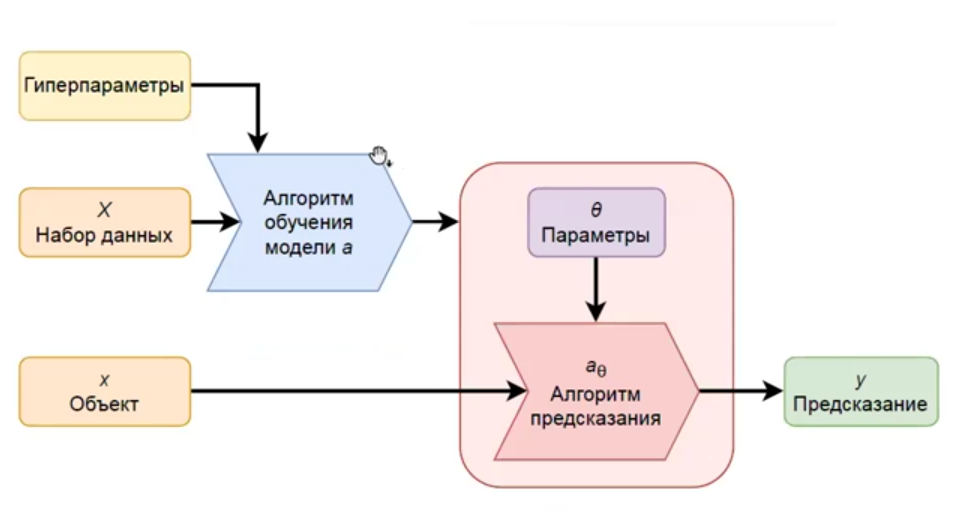
\includegraphics[scale=0.25]{Images/ml_scheme.png}
    \end{figure}\noindent
    Мы хотим сделать алгоритм предсказания, который по объекту делает предсказания. Но тут у нас параметры нам даёт не пользователь, а мы делаем их сами. А точнее, пишем специальный алгоритм (алгоритм обучения), который их нам и сделает. И это уже обычный алгоритм, с обычным входом и выходом. Его вход~--- набор данных, его выход~--- параметры алгоритма предсказания, а его параметры называются специальным словом <<\textbf{гиперпараметры}>>. То есть параметры~--- это параметры модели, которые меняются в процессе обучения, а гиперпараметры~--- фиксированные параметры алгоритма обучения.\\
    Пример: аппроксимация полиномом. Мы решили, что наш алгоритм предсказания будет выглядеть как
    \[
    y=a+bx+cx^2+dx^3+\cdots
    \]
    Где $x$~--- вход, $y$~--- выход, а $a,b,c,d,\ldots$~--- параметры. И для обучения мы себе выбрали, что будем искать только полиномы размерности 2. Тогда вот это вот <<2>>~--- гиперпараметр, точки~--- набор данных, а $a,b,c,0,0,\ldots$ будут нашими параметрами.
    \subparagraph{Уровни модельности алгоритмов.}
    \begin{enumerate}
        \item \textbf{Безмодельные алгоритмы} (<<in-place>>) решают задачу без явного построения модели. Самый тупой пример~--- нахождение матожидания и использование его как результат всех предсказаний. То есть in-place алгоритм не имеет обучения и параметров, он просто запоминает данные и гиперпараметры, и сразу на основе них делает предсказание.
        \item \textbf{Моделирующие алгоритмы} обучаются один раз и строят модель, которую потом можно переиспользовать без повторного обучения, но нельзя обновить при поступлении новых данных. Пример~--- алгоритмы кластеризации.
        \item \textbf{Алгоритмы онлайн-обучения} имеют возможность переобучаться при добавлении новых данных.
        \item Возможность объединить две модели.
    \end{enumerate}
    \paragraph{Определение понятий машинного обучения.}
    Непонятно, что называть решением задачи машинного обучения: алгоритм обучения модели, обученную модель или результат ее применения? Также непонятно, от чего вычисляется функция оценки качества: от алгоритма, от модели или от ее применения. Ответ: зависит от ситуации. Обозначим за $A$ алгоритм обучения, за $\theta$~--- полученные в результате обучения параметры, за $a_{\theta}$~--- полученную в результате обучения модель с параметрами $\theta$. Введем следующие функции оценки качества:
    \begin{enumerate}
        \item $\mathcal{L}(A,\mathcal{D})$~--- функция от алгоритма обучения
        \item $\mathcal{L}_{\mathcal{D}}(a_{\theta})$~--- функция от обученной модели
        \item $\mathcal{L}(\hat{y}, y)$, $\hat{y}=a_{\theta}(x)$~--- функция для результата применения, то есть отклонение истинного результата от предсказанного обученной моделью
    \end{enumerate}
    Очевидно, нам хочется, имея одну из этих функций, вычислять остальные. Поэтому введем три понятия:
    \begin{enumerate}
        \item \textbf{Валидация}~--- вычисление $\mathcal{L}(A,\mathcal{D})$ из $\mathcal{L}_{\mathcal{D}}(a_{\theta})$.
        \item \textbf{Тестирование модели} $a_{\theta}$ на наборе данных $\mathcal{D}$~--- вычисление $\mathcal{L}_{\mathcal{D}}(a_{\theta})$ из $\mathcal{L}(\hat{y},y)$.
        \item \textbf{Применение}~--- вычисление $a_{\theta}(x)$.
    \end{enumerate}
    \subparagraph{Валидация на отложенных данных.}
    Пусть мы хотим понять обобщающую способность нашей модели, но у нас есть ограниченный набор данных. Мы хотим убедиться, что наша модель будет выдавать хорошие результаты за пределами датасета, на котором ее обучали (для этого мы ее и обучаем). Обычно в таких случаях исходный датасет разбивают на training и test часть случайным образом. (Вообще, необязательно случайным; например, если объекты могут составить временной ряд, то разбивать объекты лучше по времени.) Тогда:
    \[\mathcal{L}(A,\mathcal{D})=\mathcal{L}(A(\mathcal{D}_{\mathrm{train}}),\mathcal{D}_{\mathrm{test}})\]
    \paragraph{Сравнение алгоритмов.}
    Чтобы сравнить в машинном обучении два алгоритма, один из которых не является частным случаем другого (тогда очевидно, что общий алгоритм лучше), нужно, во-первых, ввести метрику их сравнения, а во-вторых сравнивать на одинаковых наборах данных. Под метрикой подразумевается уже знакомая нам функция качества от алгоритма $\mathcal{L}(A,\mathcal{D})$, а также способ ее вычисления. Часто при решении задачи берут какой-то наивный алгоритм (baseline) и сравнивают остальные алгоритмы с ним. Теорема <<No free lunch theorem>> гласит, что алгоритм может работать хорошо только на определенном наборе данных, а на остальных данных проседает, т.е. нельзя покрыть одним алгоритмом все, нужно выбирать исходя набора данных в данной задаче. Лучший алгоритм для конкретной задачи с конкретным набором данных и конкретной метрикой называется State-of-the-art (SOTA).
    \paragraph{Стандартные задачи машинного обучения.}
    \begin{figure}[H]
        \begin{tabularx}{0.8\textwidth}{|X|XXX|}
            \hline
            $a\colon X\to Y$ & $Y=\{y_1,\ldots,y_k\}$ & $Y=\operatorname{Pr}^k$ & $Y=\mathbb R^k$\\
            \hline
            Обучение с учителем & Классификация & Мягкая классификация & Восстановление регрессии\\
            \hline
            One-class classification & Поиск аномалий & Восстановление плотности & {\color{red}Генерация объектов}\\
            \hline
            Обучение без учителя & Кластеризация & Мягкая кластеризация & Выделение признаков\\
            \hline
        \end{tabularx}
    \end{figure}\noindent
    Что здесь происходит? Задачу машинного обучения можно представить как отображение из $X$ в $Y$.
    В качестве столбцов у нас то, что может быть результатом:
    \begin{itemize}
        \item $Y=\{c_1,c_2,...,c_n\}$: результатом является сопоставление класса каждому объекту из набора. 
        \item $Y=\operatorname{Pr}^k$: результатом является сопоставление вектора вероятностей размера $k$ каждому объекту из набора.
        \item $Y=\mathbb{R}^k$: результатом является одно число или вектор чисел размера $k$.
    \end{itemize}
    В качестве строк выступает то, что служит источником для построения модели:
    \subparagraph{Обучение с учителем}
    В качестве источника выступают размеченные данные, то есть выборка, содержащая верные ответы. Цель алгоритма~--- научится эти правильные ответы предсказывать.
    \begin{itemize}
        \item \textbf{Задача классификации}~--- задача сопоставления каждому объекту категории на основе распределения по категориям в обучающем датасете. Наивное решение~--- всегда брать моду (самый популярный класс). Примеры: определить, является и письмо спамом или определить, какая цифра на картинке.
        \item \textbf{Задача мягкой классификации}~--- задача сопоставления объекту вектора, где каждое число обозначает уверенность в попадании объекта в конкретный класс. Выделяют вероятностную классификацию, где вектор должен быть корректным вероятностным вектором.
        \item \textbf{Задача восстановления регрессии}~--- задача предсказания ответа для произвольного объекта на основе сопоставления ответов объектам в обучающем датасете. Наивное решение~--- брать мат. ожидание.
    \end{itemize}
    Ещё в случае обучения с учителем $Y$ может быть перестановкой или рангом. В таком случае мы пытается установить порядок на наших объектах. Используется это крайне редко.\\
    Особняком стоят задачи прогнозирования временных рядов, где при имеющихся $y_{t-m},\ldots,y_{t-2},y_{t-1}$ надо предсказать $y_t$. Самый яркий пример~--- цены акций. Особняком они потому, что у них нет признаков (кроме, собственно, $y_t$). Где такие взять? Ну, например, считать, что
    \[
    x_t=(y_{t-m},\ldots,y_{t-2},y_{t-1})
    \]
    Это называется авторегрессия. Или можно брать какую-то функцию от $t$, это конструирование признаков. Наивное решение~--- арифметическое скользящее среднее или экспоненциально скользящее среднее.
    \begin{figure}[H]
        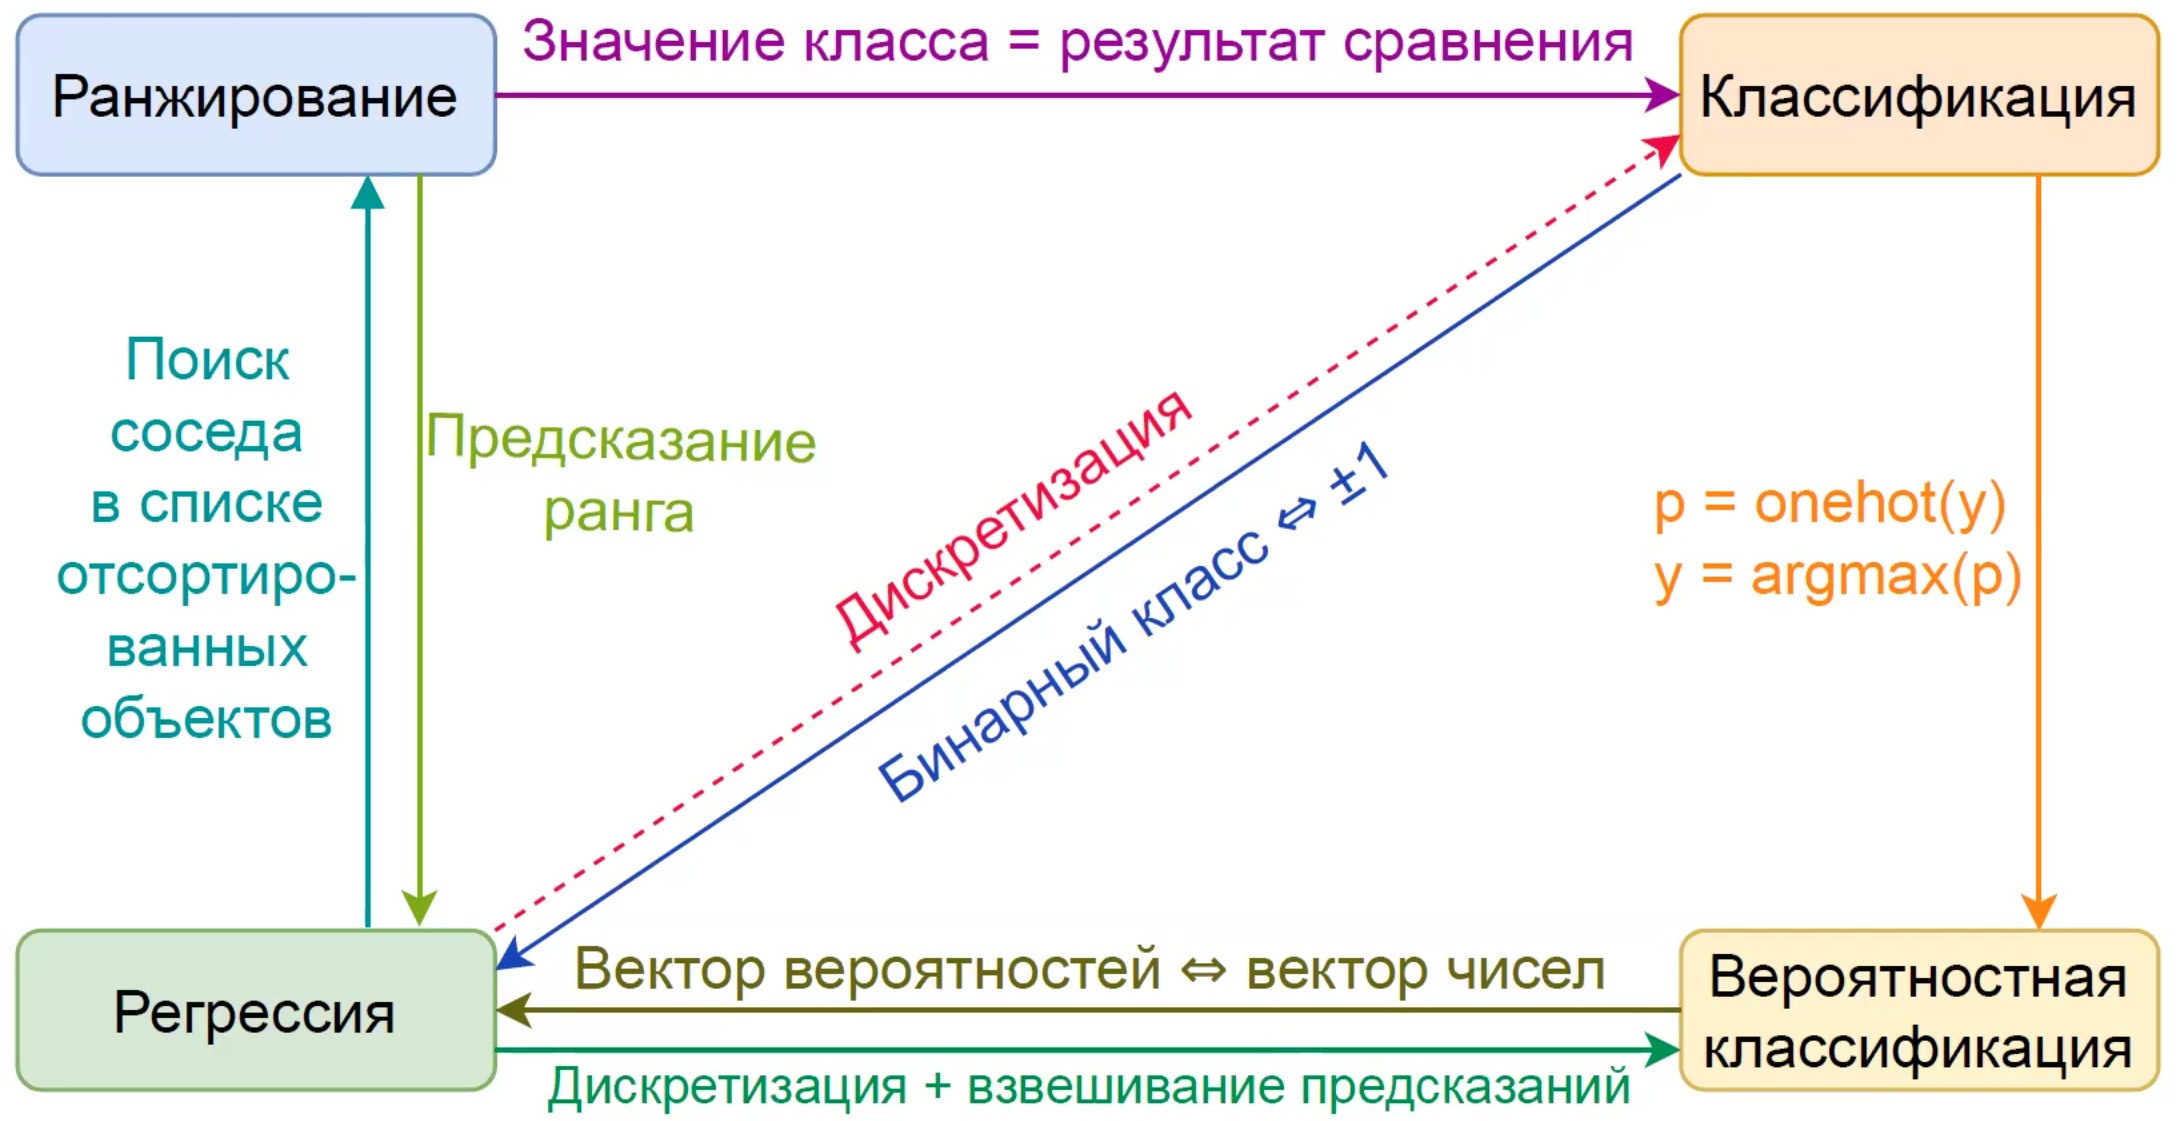
\includegraphics[width=0.7\linewidth]{Images/Supervised-learning-problem-convertions}
    \end{figure}\noindent
    \subparagraph{One-class classification}
    В качестве источника выступают данные, почти все из которых принадлежит одному классу (известно для каждого объекта, принадлежит он или нет).
    \begin{itemize}
        \item \textbf{Задача поиска аномалий}~--- среди существующих объектов нужно найти объекты другого класса.
        \item \textbf{Задача новизны}~--- среди каких-то новых объектов нужно найти объекты другого класса.
        \item \textbf{Задача восстановления плотности}~--- требуется восстановить плотность распределения и для новых объектов определить, кто из них выбивается из распределения. Обычно используется метод максимального правдоподобия, где мы оцениваем параметры распределения на основе объектов из выборки. Подробнее~--- на матстате.
        \item \textbf{Задача генерации новых объектов}~--- по данным объектам нужно сгенерировать новые.
    \end{itemize}
    Не путайте генерацию с сэмплированием (выбрать объект из существующих) и аугментацией (примитивными аналитическими операциями сгенерировать новые объекты, например, повернуть картинку котика, чтобы получить новую картинку котика). Это другие вещи, но их можно использовать как наивное решение.\\
    Из интересного, чтобы оценить качество генерации используются алгоритмы классификации (на два класса: реальный объект или сгенерированный). А ещё можно сохранять некоторую статистику между реальными объектами, тогда классификация разделяется на два вида моделей:
    \begin{itemize}
        \item Генеративные~--- обучают совместное распределение вероятностей, и задача классификации сводится к задаче восстановления плотности.
        \item Дискриминативные~--- обучают условное распределение, и модель пытается найти разделяющее правило.
    \end{itemize}
    Обычно используются в паре, но об этом подробнее во втором семестре.
    \subparagraph{Обучение без учителя.}
    В качестве источника выступают неразмеченные данные, для которых требуется самостоятельно придумать целевой признак $\widehat Y$. И дальше уже распределение на задачи ведётся в зависимости от того, каким является наш $\widehat Y$ (а не $Y$, как было в таблице).
    \begin{itemize}
        \item \textbf{Задача кластеризации}~--- требуется разделить объекты на подмножества (кластеры), чтобы в каждом кластере объекты были максимально похожи друг на друга. Пример: вы пишете Твиттер, и хотите разделить пользователей по информационным пузырям.
        \item \textbf{Задача мягкой кластеризации}~--- аналогично мягкой классификации.
        \item \textbf{Задача выделения признаков}~--- алгоритм должен отображать объект из $X$ в пространство (чаще всего меньшей размерности), которое он сам и придумает. Самое наивное~--- умножим на рандомную матрицу. Используется для уменьшения размерности, чтобы, например, нарисовать наши данные.
        \item \textbf{Задача конструирования признаков}~--- по сути, более общая задача извлечения признаков: дана какая-то абстрактная штука (картинка, текст, etc), хочется сделать себе вектор признаков. Решается явно, а не алгоритмами ML. Пример: пытаемся наложить шаблон на изображения, суммируем по всем возможным наложениям. Получаем новый признак для каждого шаблона. А вот шаблоны уже можно искать машинным обучением.
    \end{itemize}
    \subparagraph{Другие задачи машинного обучения.}
    \begin{itemize}
        \item Можно не только принимать на вход пропуски, но и возвращать. Трактуется как отказ от классификации/кластеризации. Первое используется в ансамблях, второе~--- в поиске аномалий.
        \item \textbf{Предсказание и заполнение пропусков}. Выберем признак с пропусками целевым, остальные заполним как-нибудь, натренируем модель на данных без пропусков, заполним пропуски результатом тестового прогона.
        \item \textbf{Коллаборативная фильтрация}. Дано множество оценок пользователями. И оценок, блин, мало (существенно меньше произведения числа пользователей и вещей). Требуется предсказать оценку данной вещи данным пользователем. Решается трудно, этим занимается специальный раздел (рекомендательные системы), очевидно, тем же алгоритмом, что заполнение пропусков, оно не решается, зато наоборот (заполнить пропуски совместной фильтрацией)~--- норм план.
        \item \textbf{Обучение на привилегированных данных}. Тренировочные данные содержат дополнительную информацию ($X'$), недоступную при тестировании. Базовое решение: либо не использовать $X'$, либо взять другую модель, которая предсказывает $X'$, и пользоваться ей, либо честно самому предсказывать и $X'$, и $Y$. Пример: предсказываем результат футбольного матча, и наши привилегированные данные~--- число красных и жёлтых карточек, например. На тестовых данных такое неизвестно.
        \item \textbf{Обучение на частично размеченных данных} (оно же \textbf{обучение с частичным привлечением учителя}). Лишь малая часть тренировочных данных (и никакая часть тестовые данные) содержит правильный ответ. Наивное решение: не использовать разметку (т.е. обучаться полностью без учителя) или не использовать неразмеченные объекты.
        \item \textbf{Активное обучение}~--- вариация на тему предыдущего. Можно задавать Оракулу вопросы о значении меток, и надо за минимум обращений к Оракулу восстановив $f\colon X\to Y$. То есть по сути надо не функцию найти даже, а стратегию выработать, как обращаться к Оракулу.
        \item Обучение с подкреплением (Reinforcement Learning). Есть агент и есть среда. Агент взаимодействует со средой, среда меняет состояние и возвращает награду. Задача: максимизировать награду. Пример: задача об одноруком бандите, он что-то знает об одноруком бандите, и должен выработать стратегию, как максимизировать выигрыш.
    \end{itemize}
\end{document}